\iffalse
This file is protected by Copyright. Please refer to the COPYRIGHT file
distributed with this source distribution.

This file is part of OpenCPI <http://www.opencpi.org>

OpenCPI is free software: you can redistribute it and/or modify it under the
terms of the GNU Lesser General Public License as published by the Free Software
Foundation, either version 3 of the License, or (at your option) any later
version.

OpenCPI is distributed in the hope that it will be useful, but WITHOUT ANY
WARRANTY; without even the implied warranty of MERCHANTABILITY or FITNESS FOR A
PARTICULAR PURPOSE. See the GNU Lesser General Public License for more details.

You should have received a copy of the GNU Lesser General Public License along
with this program. If not, see <http://www.gnu.org/licenses/>.
\fi

%----------------------------------------------------------------------------------------
% Required document specific properties
%----------------------------------------------------------------------------------------
\def\comp{metadata\_{}stressor}
\edef\ecomp{metadata_stressor}
\def\Comp{Metadata Stressor}
\def\docTitle{\Comp{} Component Data Sheet}
\def\snippetpath{../../../../../doc/av/tex/snippets}
%----------------------------------------------------------------------------------------
% Global latex header (this must be after document specific properties)
%----------------------------------------------------------------------------------------
\iffalse
This file is protected by Copyright. Please refer to the COPYRIGHT file
distributed with this source distribution.

This file is part of OpenCPI <http://www.opencpi.org>

OpenCPI is free software: you can redistribute it and/or modify it under the
terms of the GNU Lesser General Public License as published by the Free Software
Foundation, either version 3 of the License, or (at your option) any later
version.

OpenCPI is distributed in the hope that it will be useful, but WITHOUT ANY
WARRANTY; without even the implied warranty of MERCHANTABILITY or FITNESS FOR A
PARTICULAR PURPOSE. See the GNU Lesser General Public License for more details.

You should have received a copy of the GNU Lesser General Public License along
with this program. If not, see <http://www.gnu.org/licenses/>.
\fi

% Sets OpenCPI Version used throughout all the docs. This is updated by
% scripts/update-release.sh when a release is being made and must not
% be changed manually.
\def\ocpiversion{v2.2.0}

\documentclass{article}
\author{}  % Force author to be blank
\date{OpenCPI Release:\ \ \ocpiversion}  % Force date to be blank and override date with version
\title{OpenCPI\\\docTitle}  % docTitle must be defined before including this file
%----------------------------------------------------------------------------------------
% Paper size, orientation and margins
%----------------------------------------------------------------------------------------
\usepackage{geometry}
\geometry{
  letterpaper,  % paper type
  portrait,     % text direction
  left=.75in,   % left margin
  top=.75in,    % top margin
  right=.75in,  % right margin
  bottom=.75in  % bottom margin
}
%----------------------------------------------------------------------------------------
% Header/Footer
%----------------------------------------------------------------------------------------
\usepackage{fancyhdr} \pagestyle{fancy}  % required for fancy headers
\renewcommand{\headrulewidth}{0.5pt}
\renewcommand{\footrulewidth}{0.5pt}
\lhead{\small{\docTitle}}
\rhead{\small{OpenCPI}}
%----------------------------------------------------------------------------------------
% Various packages
%----------------------------------------------------------------------------------------
\usepackage{amsmath}
\usepackage[page,toc]{appendix}  % for appendix stuff
\usepackage{enumitem}
\usepackage{graphicx}   % for including pictures by file
\usepackage{hyperref}   % for linking urls and lists
\usepackage{listings}   % for coding language styles
\usepackage{pdflscape}  % for landscape view
\usepackage{pifont}     % for sideways table
\usepackage{ragged2e}   % for justify
\usepackage{rotating}   % for sideways table
\usepackage{scrextend}
\usepackage{setspace}
\usepackage{subfig}
\usepackage{textcomp}
\usepackage[dvipsnames,usenames]{xcolor}  % for color names see https://en.wikibooks.org/wiki/LaTeX/Colors
\usepackage{xstring}
\uchyph=0  % Never hyphenate acronyms like RCC
\renewcommand\_{\textunderscore\allowbreak}  % Allow words to break/newline on underscores
%----------------------------------------------------------------------------------------
% Table packages
%----------------------------------------------------------------------------------------
\usepackage[tableposition=top]{caption}
\usepackage{float}
\floatstyle{plaintop}
\usepackage{longtable}  % for long possibly multi-page tables
\usepackage{multicol}   % for more advanced table layout
\usepackage{multirow}   % for more advanced table layout
\usepackage{tabularx}   % c=center,l=left,r=right,X=fill
% These define tabularx columns "C" and "R" to match "X" but center/right aligned
\newcolumntype{C}{>{\centering\arraybackslash}X}
\newcolumntype{M}[1]{>{\centering\arraybackslash}m{#1}}
\newcolumntype{P}[1]{>{\centering\arraybackslash}p{#1}}
\newcolumntype{R}{>{\raggedleft\arraybackslash}X}
%----------------------------------------------------------------------------------------
% Block Diagram / FSM Drawings
%----------------------------------------------------------------------------------------
\usepackage{tikz}
\usetikzlibrary{arrows,decorations.markings,fit,positioning,shapes}
\usetikzlibrary{automata}  % used for the fsm
\usetikzlibrary{calc}      % for duplicating clients
\usepgfmodule{oo}          % to define a client box
%----------------------------------------------------------------------------------------
% Colors Used
%----------------------------------------------------------------------------------------
\usepackage{colortbl}
\definecolor{blue}{rgb}{.7,.8,.9}
\definecolor{ceruleanblue}{rgb}{0.16, 0.32, 0.75}
\definecolor{cyan}{rgb}{0.0,0.6,0.6}
\definecolor{darkgreen}{rgb}{0,0.6,0}
\definecolor{deepmagenta}{rgb}{0.8, 0.0, 0.8}
\definecolor{maroon}{rgb}{0.5,0,0}
%----------------------------------------------------------------------------------------
% Define where to hyphenate
%----------------------------------------------------------------------------------------
\hyphenation{Cent-OS}
\hyphenation{install-ation}
%----------------------------------------------------------------------------------------
% Define Commands & Rename Commands
%----------------------------------------------------------------------------------------
\newcommand{\code}[1]{\texttt{#1}}  % For inline code snippet or command line
\newcommand{\sref}[1]{Section~\ref{#1}}  % To quickly reference a section
\newcommand{\todo}[1]{\textcolor{red}{TODO: #1}\PackageWarning{TODO:}{#1}}  % To do notes
\renewcommand{\contentsname}{Table of Contents}
\renewcommand{\listfigurename}{List of Figures}
\renewcommand{\listtablename}{List of Tables}

% This gives a link to gitlab.io document. By default, it outputs the filename.
% You can optionally change the link, e.g.
% \githubio{FPGA\_Vendor\_Tools\_Installation\_Guide.pdf} vs.
% \githubio[\textit{FPGA Vendor Tools Installation Guide}]{FPGA\_Vendor\_Tools\_Installation\_Guide.pdf}
% or if you want the raw ugly URL to come out, \githubioURL{FPGA_Vendor_Tools_Installation_Guide.pdf}
\newcommand{\githubio}[2][]{% The default is for FIRST param!
\href{http://opencpi.gitlab.io/releases/\ocpiversion/docs/#2}{\ifthenelse{\equal{#1}{}}{\texttt{#2}}{#1}}}
\newcommand{\gitlabcom}[2][]{% The default is for FIRST param!
\href{http://gitlab.com/opencpi/#2}{\ifthenelse{\equal{#1}{}}{\texttt{#2}}{#1}}}
\newcommand{\githubioURL}[1]{\url{http://opencpi.gitlab.io/releases/\ocpiversion/docs/#1}}
% Lastly, if you want a SINGLE leading path stripped, e.g. assets/X.pdf => X.pdf:
\newcommand{\githubioFlat}[1]{%
\StrBehind{#1}{/}[\den]%
\href{http://opencpi.gitlab.io/releases/\ocpiversion/docs/#1}{\texttt{\den}}%
}
%----------------------------------------------------------------------------------------
% VHDL Coding Language Style
% modified from: http://latex-community.org/forum/viewtopic.php?f=44&t=22076
%----------------------------------------------------------------------------------------
\lstdefinelanguage{VHDL}
{
  basicstyle=\ttfamily\footnotesize,
  columns=fullflexible,keepspaces,  % https://tex.stackexchange.com/a/46695/87531
  keywordstyle=\color{ceruleanblue},
  commentstyle=\color{darkgreen},
  morekeywords={
    library, use, all, entity, is, port, in, out, end, architecture, of,
    begin, and, signal, when, if, else, process, end,
  },
  morecomment=[l]--
}
%----------------------------------------------------------------------------------------
% XML Coding Language Style
% modified from http://tex.stackexchange.com/questions/10255/xml-syntax-highlighting
%----------------------------------------------------------------------------------------
\lstdefinelanguage{XML}
{
  basicstyle=\ttfamily\footnotesize,
  columns=fullflexible,keepspaces,
  morestring=[s]{"}{"},
  morecomment=[s]{!--}{--},
  commentstyle=\color{darkgreen},
  moredelim=[s][\color{black}]{>}{<},
  moredelim=[s][\color{cyan}]{\ }{=},
  stringstyle=\color{maroon},
  identifierstyle=\color{ceruleanblue}
}
%----------------------------------------------------------------------------------------
% DIFF Coding Language Style
% modified from http://tex.stackexchange.com/questions/50176/highlighting-a-diff-file
%----------------------------------------------------------------------------------------
\lstdefinelanguage{diff}
{
  basicstyle=\ttfamily\footnotesize,
  columns=fullflexible,keepspaces,
  breaklines=true,                            % wrap text
  morecomment=[f][\color{ceruleanblue}]{@@},  % group identifier
  morecomment=[f][\color{red}]-,              % deleted lines
  morecomment=[f][\color{darkgreen}]+,        % added lines
  morecomment=[f][\color{deepmagenta}]{---},  % Diff header lines (must appear after +,-)
  morecomment=[f][\color{deepmagenta}]{+++},
}
%----------------------------------------------------------------------------------------
% Python Coding Language Style
%----------------------------------------------------------------------------------------
\lstdefinelanguage{python}
{
  basicstyle=\ttfamily\footnotesize,
  columns=fullflexible,keepspaces,
  keywordstyle=\color{ceruleanblue},
  commentstyle=\color{darkgreen},
  stringstyle=\color{orange},
  morekeywords={
    print, if, sys, len, from, import, as, open,close, def, main, for, else,
    write, read, range,
  },
  comment=[l]{\#}
}
%----------------------------------------------------------------------------------------
% Fontsize Notes in order from smallest to largest
%----------------------------------------------------------------------------------------
%    \tiny
%    \scriptsize
%    \footnotesize
%    \small
%    \normalsize
%    \large
%    \Large
%    \LARGE
%    \huge
%    \Huge

\graphicspath{{figures/}}
%----------------------------------------------------------------------------------------

\begin{document}
\maketitle
\thispagestyle{empty}
\newpage

\def\name{\comp}
\def\workertype{Application}
\def\version{\ocpiversion}
\def\releasedate{9/2018}
\def\componentlibrary{ocpi.core}
\def\workers{\comp{}.hdl, \comp{}.rcc}
\def\testedplatforms{alst4, centos6, centos7, isim, Matchstiq-Z1(PL), ml605, modelsim, xilinx13\_{}3, xsim, ZedBoard(PL)}
\section*{Summary - \Comp}
\begin{tabular}{|c|M{13.5cm}|}
  \hline
  \rowcolor{blue}
   & \\
  \hline
  Name              & \comp             \\
  \hline
  Worker Type       & \workertype       \\
  \hline
  OpenCPI Release   & \ocpiversion      \\
  \hline
  Last Update       & \releasedate      \\
  \hline
  Component Library & \componentlibrary \\
  \hline
  Workers           & \workers          \\
  \hline
  Tested Platforms  & \testedplatforms  \\
  \hline
\end{tabular}


\section*{Functionality}
\begin{flushleft}
The \textit{\comp} component tests an HDL worker's robustness during development as part of the unit test suite. An HDL worker is expected to accept all valid combinations of metadata without failure, though some are unlikely to be encountered in normal operation. It also may starve the unit under test of data and insert delays between messages. The data starvation may be random or based on a duty cycle. The worker is automatically built into the HDL test assemblies generated by the framework. It can also add zero length messages between messages. It passes through the data it receives without change.  \medskip
\end{flushleft}


\section*{Worker Implementation Details}
\subsection*{\comp.hdl}
\begin{flushleft}
The \textit{\comp} test worker has four modes controlling its primary operation: bypass, data, metadata, and full. In bypass mode, this worker passes through the data and metadata it receives without change. In data mode, the worker passes through the metadata associated with a message unchanged, but the data will be withheld based on the duty cycle or lfsr, imitating data starvation for the unit under test. (If enable\_take\_lsfr is not set to true or take\_duty is not set to greater than 1, then the worker will set the duty cycle to 5.) In metadata mode, the worker passes through the data (not intentionally withholding any data) but manipulates the metadata in the following ways:
\begin{itemize}
 \item early start of message (SOM), data, late end of message (EOM)
 \item early SOM, data, EOM with data
 \item SOM with data, data, late EOM
 \item SOM with data, data, EOM with data, (single word message if that is what is received)
 \item zero length message (if allow\_zlms is true)
\end{itemize}
It repeats those patterns so long as there is data.
In full mode, the worker combines data and metadata modes, manipulating both the metadata and starving the unit under test of data.
Do not use data and allow\_zlms in combination. Data mode does not allow for manipulation of metadata, so zero length messages cannot be inserted. Enabling both does not cause a failure, but one behavior will preclude the expression of the other.  \medskip
\end{flushleft}

\subsection*{\comp.rcc}
\begin{flushleft}
The RCC version of this component is just a placeholder to fulfill the requirements of unit test framework. It passes through data without change and shouldn't be included in normal applications, as it provides no real functionality.  \medskip
\end{flushleft}

\section*{Theory}
\begin{flushleft}
There are some combinations of metadata that are valid but not often encountered that a worker should be able to handle without failure.   \medskip
\end{flushleft}

\section*{Block Diagrams}
\subsection*{Top level}
\begin{center}
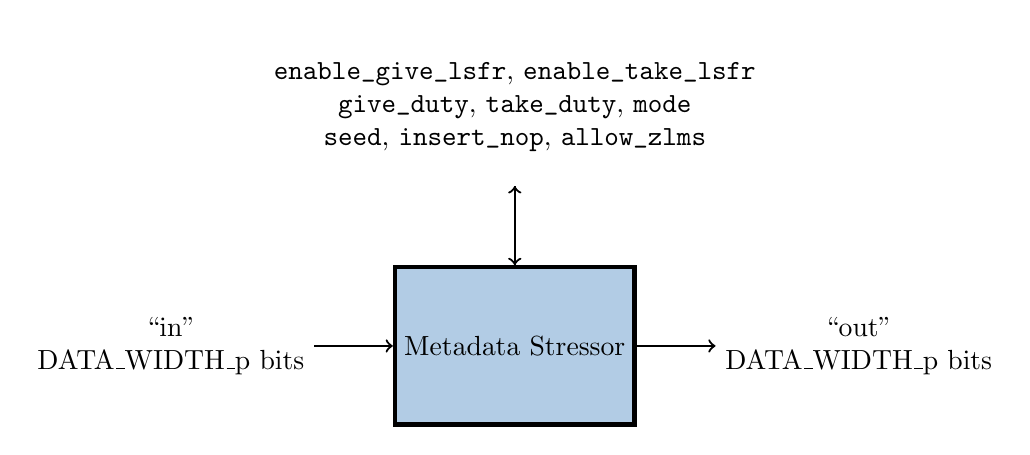
\begin{tikzpicture}[% List of styles applied to all, to override specify on a case-by-case
	every node/.style={
		align=center,  		% use this so that the "\\" for line break works
		minimum size=2cm	% creates space above and below text in rectangle
		},
		every edge/.style={draw,thick}
		]
	\node[rectangle,ultra thick,draw=black,fill=blue](R2){\Comp};
	\node[rectangle,draw=white,fill=white](R3)[left= of R2]{``in'' \\ DATA\_WIDTH\_p bits};
	\node[rectangle,draw=white,fill=white](R4)[right= of R2]{``out'' \\ DATA\_WIDTH\_p bits};
	\node[rectangle,draw=white,fill=white](R5)[above= of R2]{\verb+enable_give_lsfr+, \verb+enable_take_lsfr+ \\ \verb+give_duty+, \verb+take_duty+, \verb+mode+ \\ \verb+seed+, \verb+insert_nop+, \verb+allow_zlms+};
	\path[->]
	(R3)edge []	node [] {} (R2)
	(R2)edge []	node [] {} (R4)
	(R2)edge []	node [] {} (R5)
	(R5)edge []	node [] {} (R2)
	;
\end{tikzpicture}
\captionof{figure}{Top Level Block Diagram}
\end{center}\pagebreak

\subsection*{State Machine}
\begin{flushleft}
Below is an abbreviated representation of the primary finite state machine implemented in the HDL version of this component.
\end{flushleft}
\begin{center}
	\centering\captionsetup{type=figure}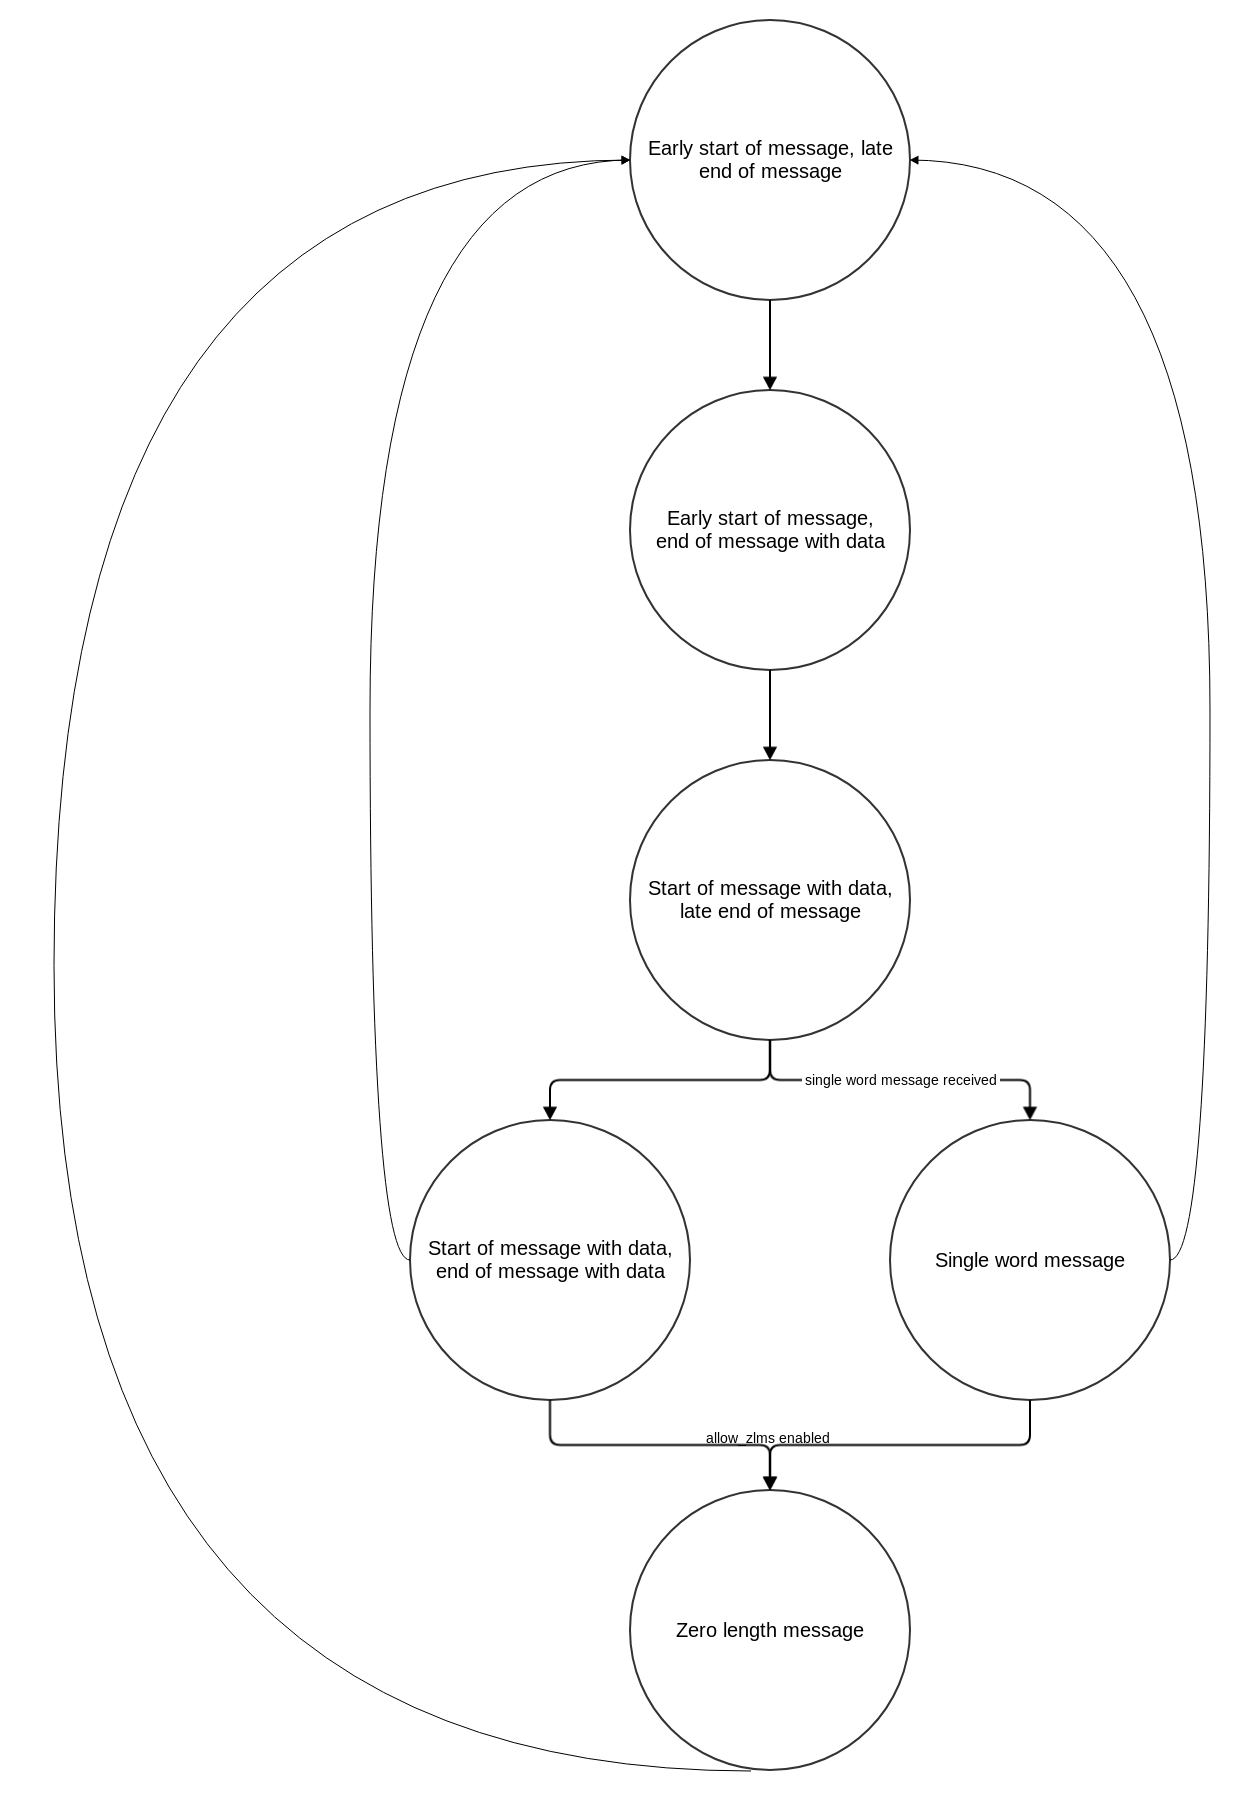
\includegraphics[scale=0.25]{ms_fsm_abrv}
\end{center}

\section*{Source Dependencies}
\subsection*{\comp.hdl}
\begin{itemize}
	\item projects/core/components//metadata\_stressor.hdl/metadata\_stressor.vhd
	\item core/hdl/primitives/util/util\_pkg.vhd
	      \subitem projects/core/hdl/primitives/util/zlm\_detector.vhd
\end{itemize}

\subsection*{\comp.rcc}
\begin{itemize}
	\item projects/core/components/metadata\_stressor.rcc/metadata\_stressor.cc
\end{itemize}

\begin{landscape}
	\section*{Component Spec Properties}
	\begin{scriptsize}
% do not delete this line, it is used by the auto gen script to insert latex code
\begin{tabular}{|p{2cm}|p{1.5cm}|c|c|c|p{1.5cm}|p{1cm}|p{7cm}|}
\hline
\rowcolor{blue}
Name & Type & SequenceLength & ArrayDimensions & Accessibility & Valid Range & Default & Usage \\
\hline
\verb+enable_give_lsfr+  & bool & - & - & Readable, Writable & Standard & False & True: MSB of lsfr drives give, False: give\_duty drives give \\
\hline
\verb+enable_take_lsfr+  & bool & -  & - & Readable, Writable & Standard & False & True: 7th bit of lsfr drives take, False: take\_duty drives take \\
\hline
\verb+give_duty+     & ushort & -  & - & Readable, Writable & Standard & 1 & Set `give' duty cycle if enable\_give\_lsfr is false \\
\hline
\verb+take_duty+     & ushort & -  & -  & Readable, Writable & Standard & 1 & Set `take' duty cycle if enable\_take\_lsfr is false \\
\hline
\verb+mode+     & enum & -  & -  & Readable, Writable & Standard & bypass & bypass: worker passes through data and metadata, data: worker varies data, but passes through metadata, metadata: vary metadata, keep data steady, full: vary all metadata and data \\
\hline
\verb+seed+     & ushort & -  & - & Readable, Writable & Standard & 1 & seed for lsfr \\
\hline
\verb+allow_zlms+     & bool & -  & -  & Readable, Writable & Standard & False & Insert ZLMs between some messages \\
\hline
\verb+insert_nop+     & bool & -  & -  & Readable, Writable & Standard & False & Insert delays between messages \\
\hline
\end{tabular}
%GEN_SPEC_TABLE
\end{scriptsize}

\section*{Worker Properties}
\subsection*{\comp.hdl}
\begin{scriptsize}
	\begin{tabular}{|p{1.5cm}|p{2.5cm}|p{1cm}|c|c|c|p{2cm}|p{1cm}|p{5cm}|}
		\hline
		\rowcolor{blue}
		Type     & Name                      & Type  & SequenceLength & ArrayDimensions & Accessibility       & Valid Range & Default & Usage                                      \\
		\hline
		Property & \verb+DATA_WIDTH_p+   & UChar & -              & -               & Readable, Parameter & 8/16/32/64        & 12      & I/O data width                   \\
		\hline
	\end{tabular}
\end{scriptsize}
% do not delete this line, it is used by the auto gen script to insert latex code
%GEN_WORKER_TABLE

\section*{Component Ports}
\begin{scriptsize}
% do not delete this line, it is used by the auto gen script to insert latex code
\begin{tabular}{|M{2cm}|M{1.5cm}|M{4cm}|c|c|M{9cm}|}
\hline
\rowcolor{blue}
Name & Producer & Protocol & Optional & Advanced & Usage
\\
\hline
in & false & None& False & - & 32 bits\\
\hline
out & true & None& False & - & 32 bits\\
\hline
\end{tabular}
%GEN_PORT_TABLE
\end{scriptsize}

\section*{Worker Interfaces}
\subsection*{\comp.hdl}
\begin{scriptsize}
	\begin{tabular}{|M{2cm}|M{1.5cm}|M{4cm}|c|M{12cm}|}
		\hline
		\rowcolor{blue}
		Type            & Name & DataWidth            & Advanced & Usage                                       \\
		\hline
		StreamInterface & in   & \verb+DATA_WIDTH_p+ & -        & Size defined by \verb+DATA_WIDTH_p+        \\
		\hline
		StreamInterface & out  & \verb+DATA_WIDTH_p+ & -        & Size defined by \verb+DATA_WIDTH_p+ \\
		\hline
	\end{tabular}
\end{scriptsize}
\end{landscape}

\section*{Control Timing and Signals}
\subsection*{\comp.hdl}
\begin{flushleft}
This worker implementation uses the clock from the Control Plane and standard Control Plane signals.
\end{flushleft}

\begin{landscape}
\section*{Worker Configuration Parameters}
\subsubsection*{\comp.hdl}
%\input{../../\ecomp.hdl/configurations.inc}
\section*{Performance and Resource Utilization}
\subsubsection*{\comp.hdl}
%\input{../../\ecomp.hdl/utilization.inc}
\end{landscape}

\section*{Test and Verification}
\begin{flushleft}
This component is tested via the unit test automation feature of the framework. The component's .test/ contains XML files that describe the combinations of tests. \medskip

The test cases exercise changes in every property across three cases, though not every property in every case, as that would take a prohibitively long time.

\begin{itemize}
\item Case 1 - Tests the component with crafted ZLMs and SWMs, backpressure on, timeout set to 120 seconds
\begin{enumerate}
	\item enable\_give\_lsfr = True: use lsfr to vary give
	\item enable\_take\_lsfr = True: use lsfr to vary take
	\item insert\_nop = True: insert delay between messages
	\item mode = full: vary data and metadata
\end{enumerate}

\item Case 2 - Tests the component with eight byte messages, backpressure on, timeout set to 120 seconds
\begin{enumerate}
	\item enable\_give\_lsfr = True: use lsfr to vary give
	\item enable\_take\_lsfr = True: use lsfr to vary take
	\item insert\_nop = True: insert delay between messages
	\item mode = full: vary data and metadata
\end{enumerate}

\item Case 3 - Tests the component with a single zlm, backpressure on, timeout set to 120 seconds
\begin{enumerate}
	\item enable\_give\_lsfr = True: use lsfr to vary give
	\item enable\_take\_lsfr = True: use lsfr to vary take
	\item insert\_nop = True: insert delay between messages
	\item mode = full: vary data and metadata
\end{enumerate}

\item Case 4 - Tests the component with crafted ZLMs and SWMs, backpressure on, timeout set to 120 seconds
\begin{enumerate}
	\item enable\_give\_lsfr = True: use lsfr to vary give
	\item enable\_take\_lsfr = True: use lsfr to vary take
	\item insert\_nop = True: insert delay between messages
  \item mode = data: only vary data
	\item mode = metadata: only vary metadata
	\item mode = full: vary data and metadata
\end{enumerate}

\item Cases 5-11 - Tests ending on different message types, message size set to 4, stressormode set to full, backpressure on, timeout set to 120 seconds
\begin{enumerate}
	\item mode = full: vary data and metadata
	\item insert\_nop = True: insert delay between messages
	\item insert\_nop = False: no delay between messages
\end{enumerate}

\item Case 12 -  Tests most of the functionality, message size set to 128, backpressure on, stressormode set to full, timeout set to 240 seconds
\begin{enumerate}
	\item enable\_give\_lsfr = True: use lsfr to vary give
	\item enable\_give\_lsfr = False: use duty cycle to vary give
	\item enable\_take\_lsfr = True: use lsfr to vary take
	\item enable\_take\_lsfr = False: use duty cycle to vary take
	\item give\_duty = 1: constant
	\item give\_duty = 4: 1 on 3 off
	\item take\_duty = 1: constant
	\item take\_duty = 5: 1 on 4 off
	\item mode = data: only vary data
	\item mode = metadata: only vary metadata
	\item mode = full: vary data and metadata
	\item insert\_nop = True: insert delay between messages
	\item insert\_nop = False: no delay between messages
	\item seed = 35: seed for lsfr
\end{enumerate}

\item Case 13 - Tests the RCC version of this component, which is nothing but a placeholder, timeout set to 120 seconds
\end{itemize}

In all test cases, the data is simply passed through the component and the tests are determined to be successful by comparing the input and output files.

\end{flushleft}
\end{document}
